\documentclass{beamer}
\usepackage[spanish]{babel}
\usepackage[utf8]{inputenc}
\usepackage{listings}
\usepackage{color}
\usepackage[T1]{fontenc}
\usepackage{pgfpages}
\usepackage{graphicx}
\DeclareGraphicsExtensions{.pdf,.png,.jpg}
\usepackage[T1]{fontenc}
\usetheme[pageofpages=of,% String used between the current page and the
          bullet=circles,% Use circles instead of squares for bullets.
          titleline=true,% Show a line below the frame title.
          alternativetitlepage=true,% Use the fancy title page.
          ]{Madrid}
\usecolortheme[RGB={220,122,40}]{structure}
\title{Instalaci\'on y Administraci\'on de Linux}
\author{Jennifer }
\date{\today}
\newtheorem{defi}{{\sc Definición}}

\begin{document}
\begin{frame}
\titlepage
\end{frame}

\setcounter{tocdepth}{1}

\begin{frame}[allowframebreaks]
\frametitle{\'Indice}
\tableofcontents
\end{frame}

\section{El Filesystem Hierarchy Standard}
\subsection{Estructura del \'arbol de directorios}
\begin{frame}
\setcounter{tocdepth}{3}
\tableofcontents[currentsection]
\frametitle{El Sistema de Archivos}
\end{frame} 

\section{El Filesystem Hierarchy Standard}
\subsection{Estructura del \'arbol de directorios}
\begin{frame}
\frametitle{El Sistema de Archivos}
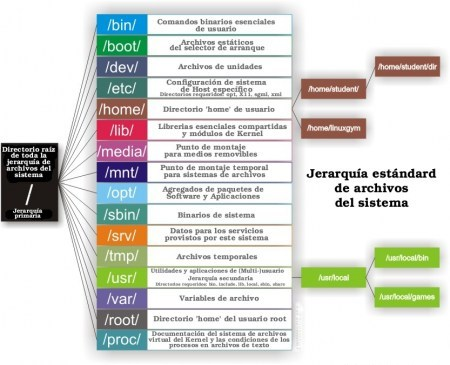
\includegraphics[height=0.8\textheight]{fhs-esp.jpg} \hspace*{7.3cm}
\end{frame} 

\section{Instalaci\'on del sistema GNU/Linux}
\subsection{Antes de Instalar...}
\begin{frame}
\frametitle{Antes de Instalar, recuerda..}
	\begin{itemize}
	\item Respalda la Data de tu computador.
	\item Necesitaras la siguiente informaci\'on: 
		\begin{itemize}
		\item Compatibilidad con el Hardware
		\item Configuraci\'on de la Red
		\item Tener el m\'inimo de requerimientos de hardware.
		\item Particionar en caso que se est\'e usando windows en otra participaci\'on.
		\end{itemize}
	\end{itemize}
\end{frame}

\subsection{Configuraci\'on general}
\begin{frame}
\tableofcontents[currentsection]
\end{frame} 


\begin{frame}
\frametitle{La Instalaci\'on}
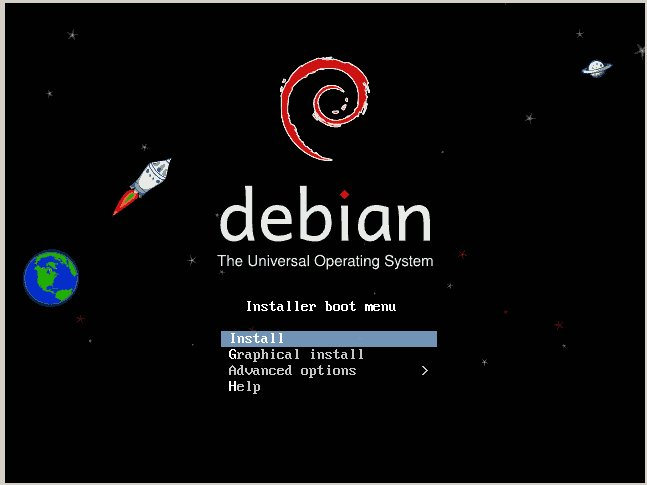
\includegraphics[height=0.8\textheight]{./imgs/1_inicioCD.jpg} \hspace*{7.3cm}
\end{frame} 

\begin{frame}
\frametitle{Esto se debe hacer antes de...}
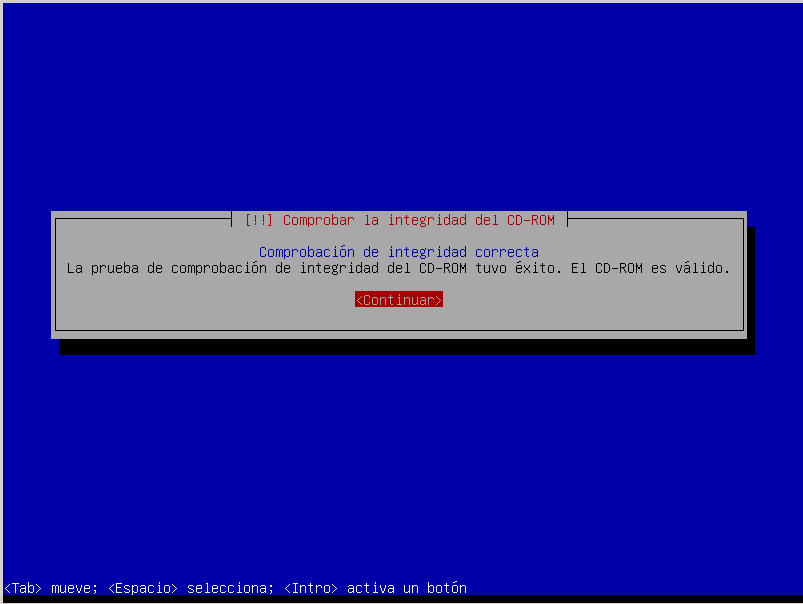
\includegraphics[height=0.8\textheight]{./imgs/5_install_comprobaciondeCD.png} \hspace*{7.3cm}
\end{frame} 

\begin{frame}
\frametitle{Opciones Avanzadas}
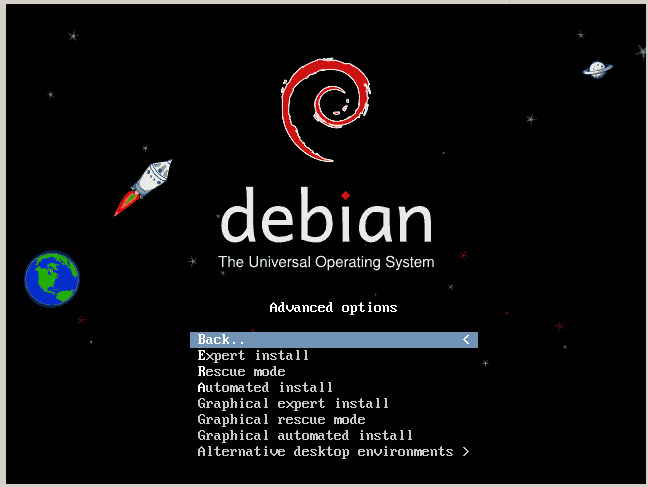
\includegraphics[height=0.8\textheight]{./imgs/3_opt_avan.png} \hspace*{7.3cm}
\end{frame}


\begin{frame}
\frametitle{Opciones Avanzadas: modo experto}
  \begin{columns}
  \column{.5\linewidth}
	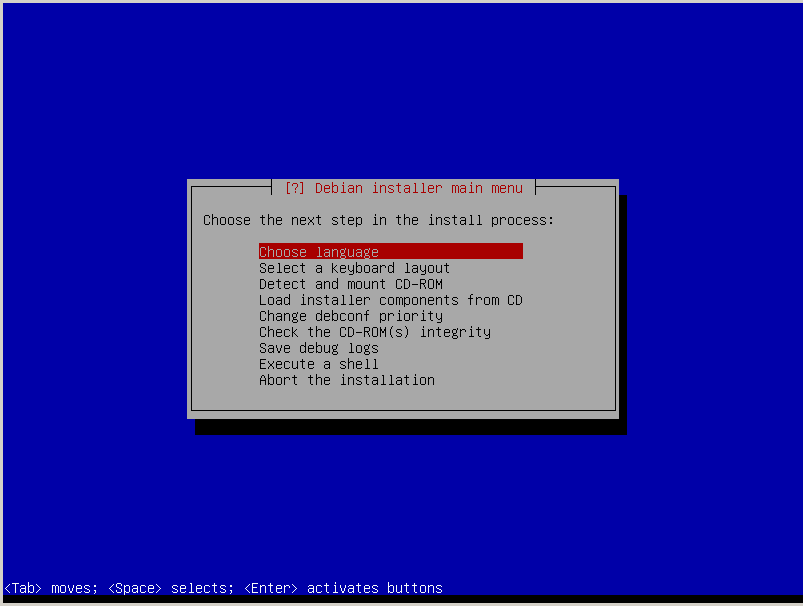
\includegraphics[width=0.9\textwidth]{./imgs/3_1_expert_install.png} \hspace*{7.3cm}
  \column{.5\linewidth}
	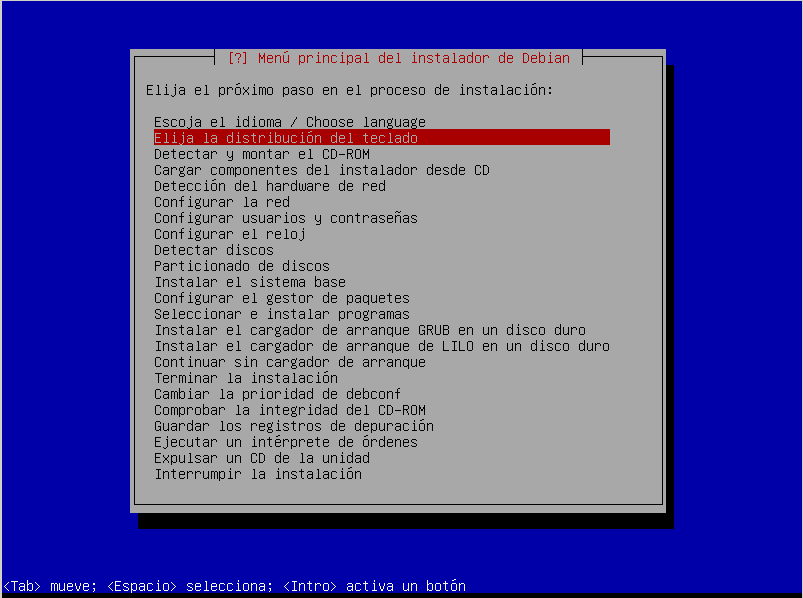
\includegraphics[width=0.9\textwidth]{./imgs/6_modo_expert.png} \hspace*{7.3cm}
  \end{columns}
\end{frame}

\begin{frame}
\frametitle{Opciones Avanzadas: modo rescate}
  \begin{columns}
  \column{.5\linewidth}
                        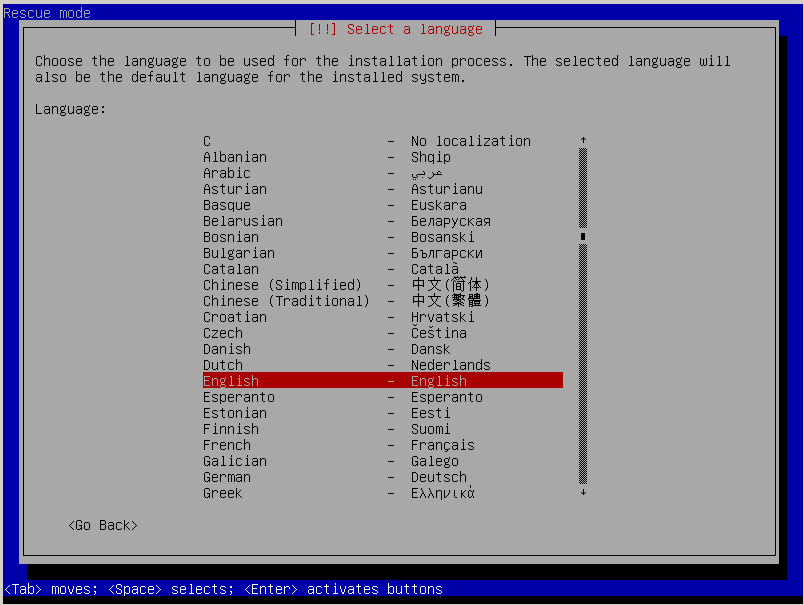
\includegraphics[ width=0.9\textwidth]{./imgs/3_2_rescue_mode.png}
  \column{.5\linewidth}
                        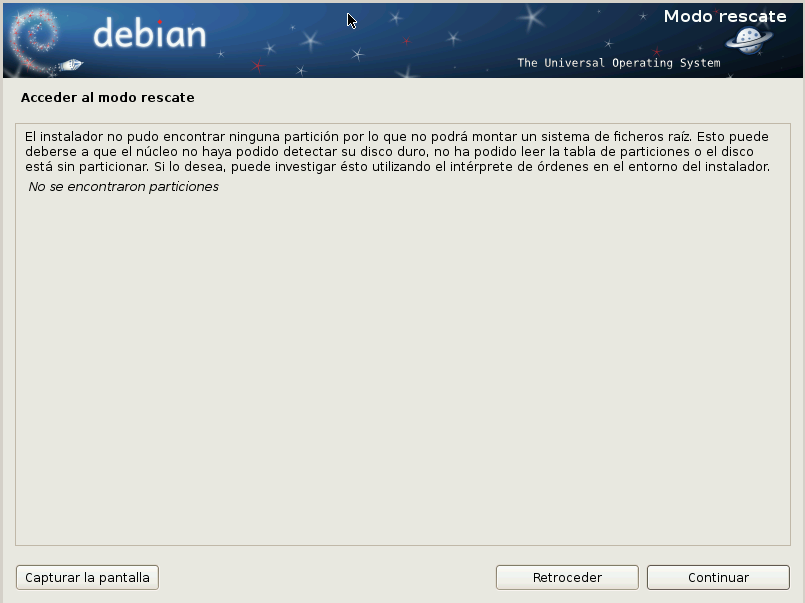
\includegraphics[ width=0.9\textwidth]{./imgs/3_2_1_modo_rescate.png}
  \end{columns}
\end{frame}

\begin{frame}
\frametitle{Opciones Avanzadas: instalaci\'on automatizada}
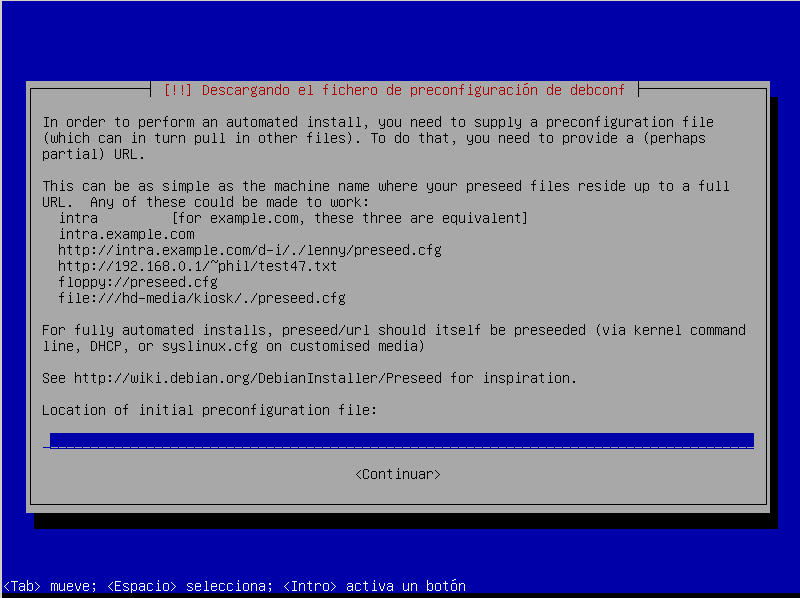
\includegraphics[ width=0.9\textwidth]{./imgs/7_automate_install.png}
\end{frame}

\begin{frame}
\frametitle{Opciones Avanzadas: otros entornos de Escritorio}
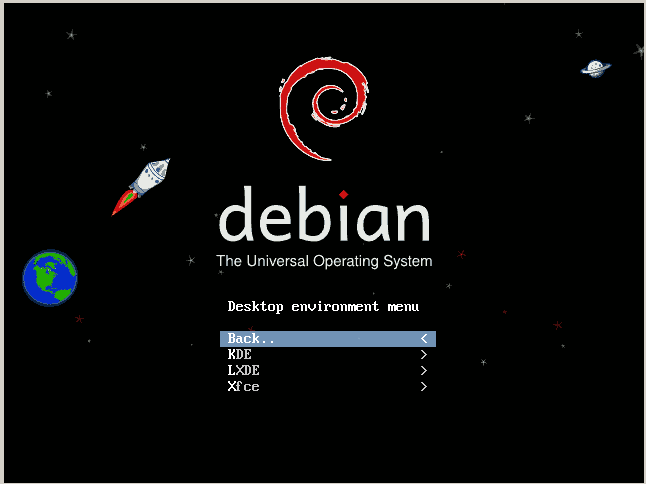
\includegraphics[height=0.8\textheight]{./imgs/3_4_alternative_desktop.png} \hspace*{7.3cm}
\end{frame}

\begin{frame}
\frametitle{La Instalaci\'on}
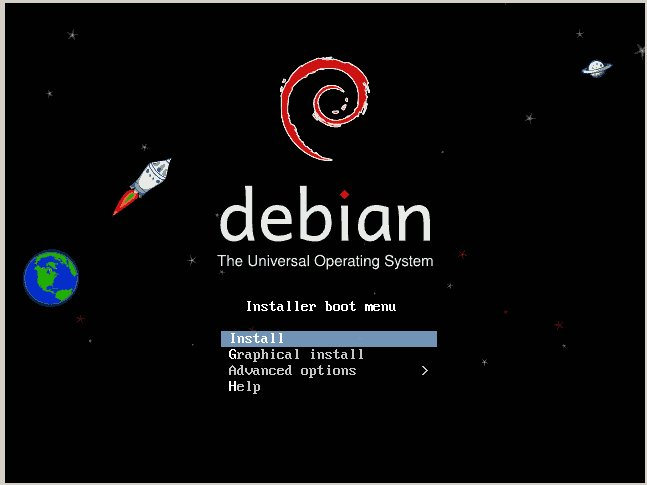
\includegraphics[height=0.8\textheight]{./imgs/1_inicioCD.jpg} \hspace*{7.3cm}
\end{frame} 

\subsection{Configuraci\'on general}
\begin{frame}
\frametitle{Escoger el Lenguaje}
  \begin{columns}
  \column{.5\linewidth}
                        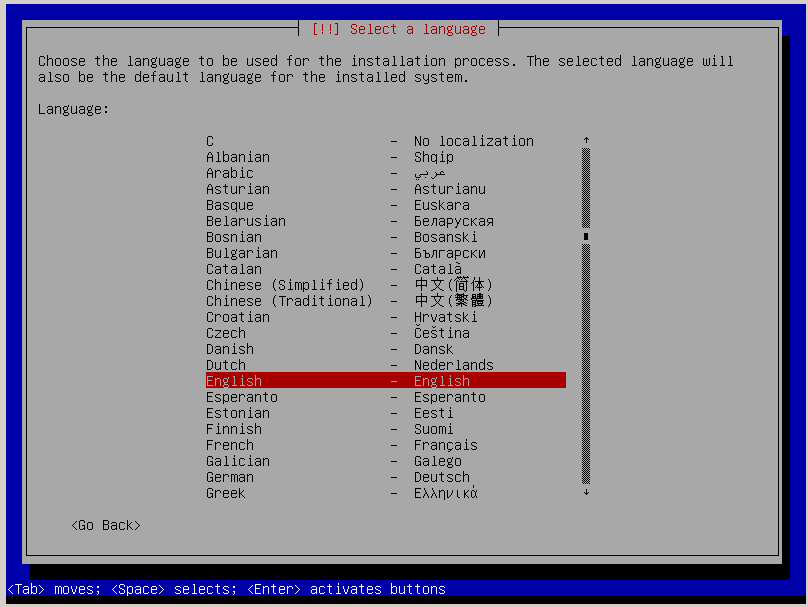
\includegraphics[ width=0.9\textwidth]{./imgs/2_lenguaje.png}
  \column{.5\linewidth}
                        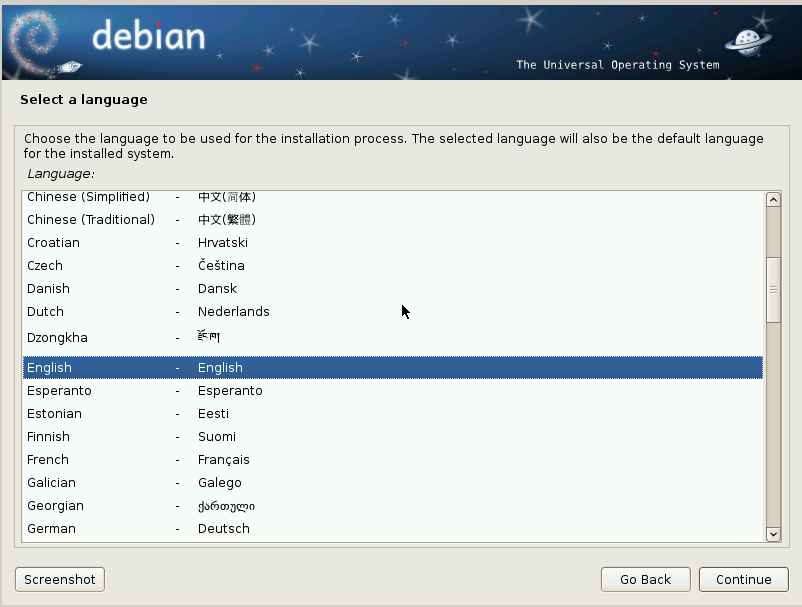
\includegraphics[ width=0.9\textwidth]{./imgs/2_lenguaje_g.png}
  \end{columns}
\end{frame} 

\subsection{Configuraci\'on general: Ubicacion y Teclado }
\begin{frame}
\frametitle{Escoger Ubicaci\'on y distribuci\'on de teclado}
  \begin{columns}
  \column{.5\linewidth}
                        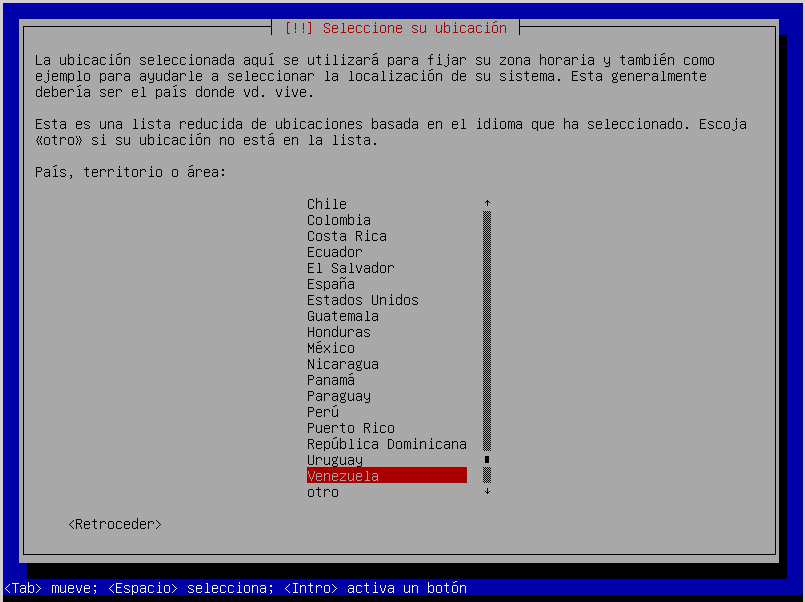
\includegraphics[ width=0.9\textwidth]{./imgs/4_1_install_ubicacion.png}
  \column{.5\linewidth}
                        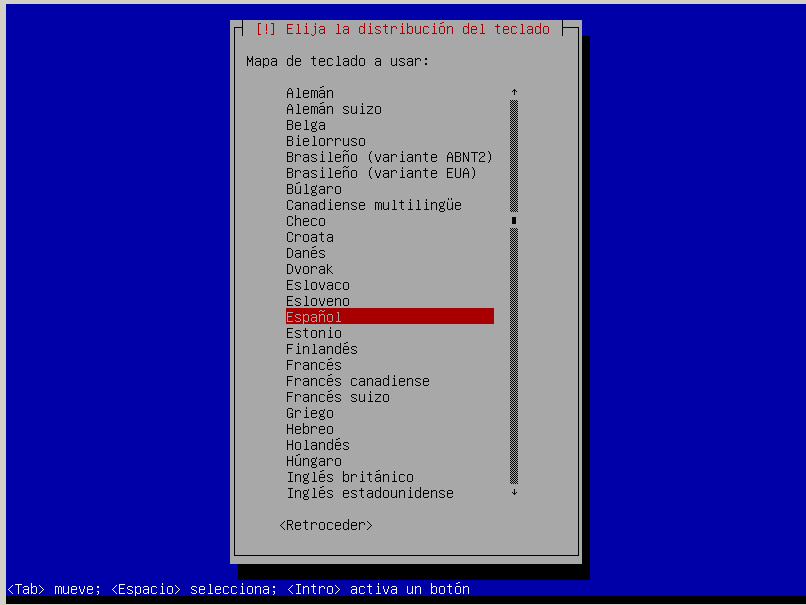
\includegraphics[ width=0.9\textwidth]{./imgs/4_2_install_distteclado.png}
  \end{columns}
\end{frame} 

\subsection{Configuraci\'on general: Nombre de la Máquina}
\begin{frame}
\frametitle{Nombre de la m\'aquina}
  \begin{columns}
  \column{.5\linewidth}
                        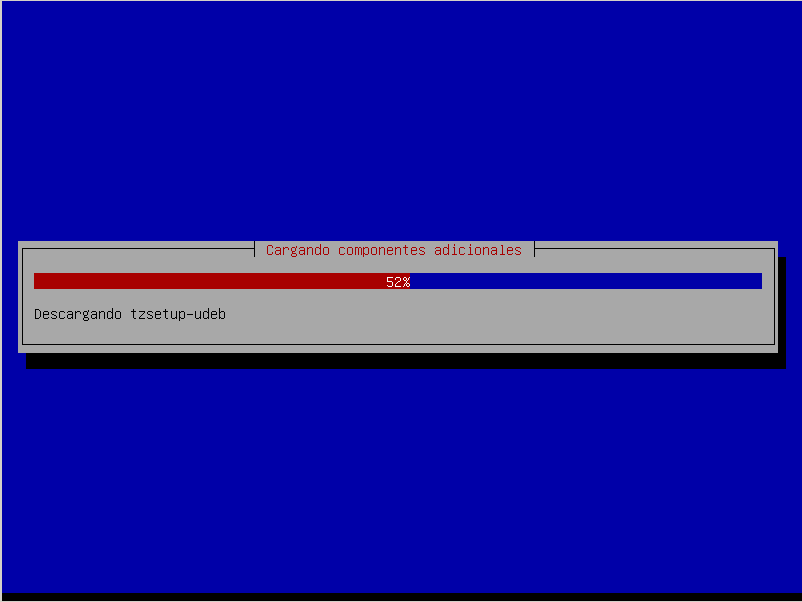
\includegraphics[ width=0.9\textwidth]{./imgs/4_3_install_load_files.png}
  \column{.5\linewidth}
                        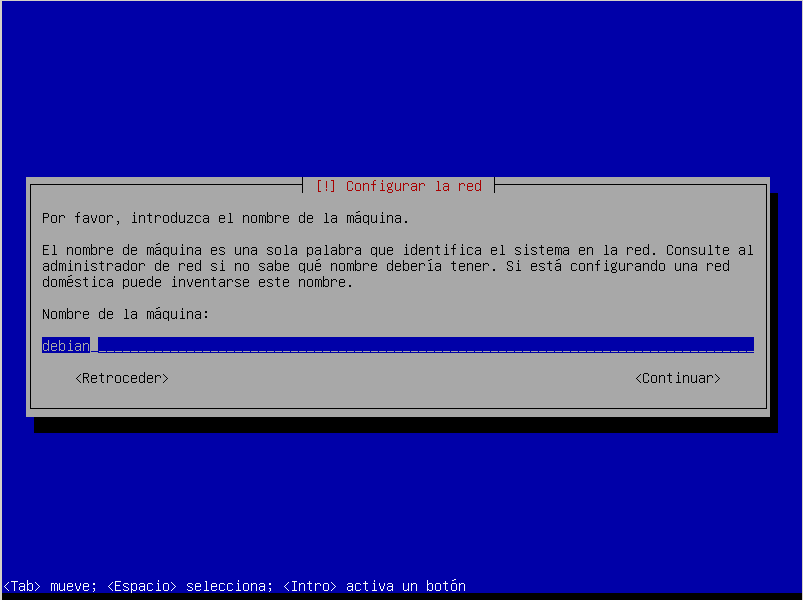
\includegraphics[ width=0.9\textwidth]{./imgs/4_4_install_nb_machine.png}
  \end{columns}
\end{frame} 

\subsection {Configuraci\'on general: Dominio y usuario Root}
\begin{frame}
\frametitle{Dominio de red y Usuario Root}
  \begin{columns}
  \column{.5\linewidth}
                        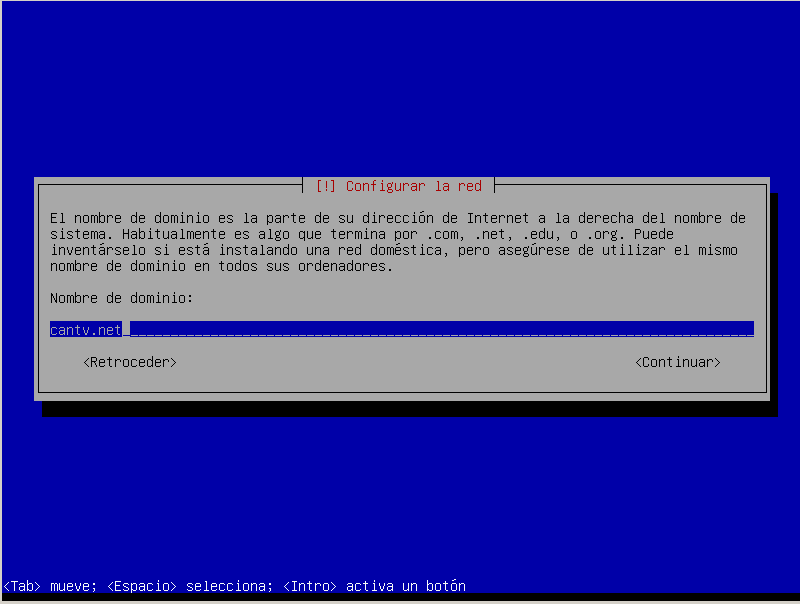
\includegraphics[ width=0.9\textwidth]{./imgs/4_5_install_dominiodered.png}
  \column{.5\linewidth}
                        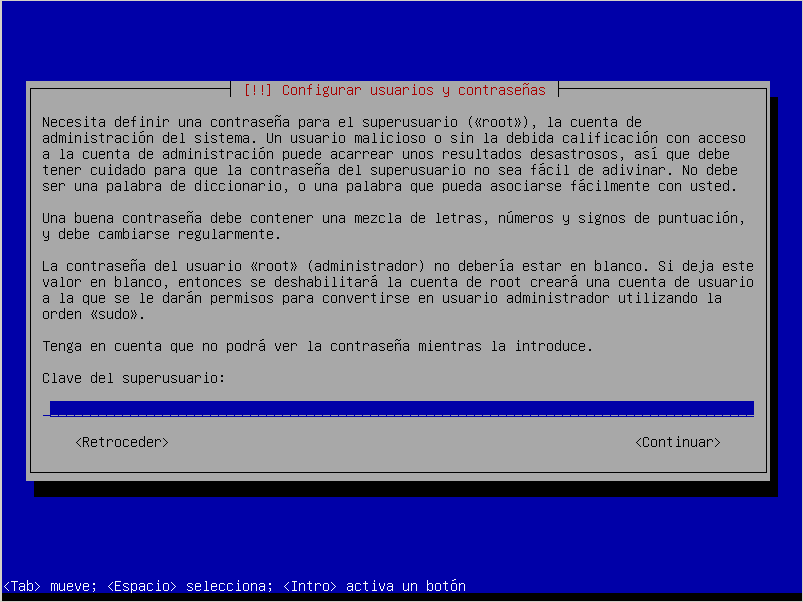
\includegraphics[ width=0.9\textwidth]{./imgs/4_6_install_configsuperuser.png}
  \end{columns}
\end{frame} 

 
\subsection{Configuraci\'on general: Usuario Personal}
\begin{frame}
\frametitle{Usuario Personal} 
  \begin{columns}
  \column{.5\linewidth}
                        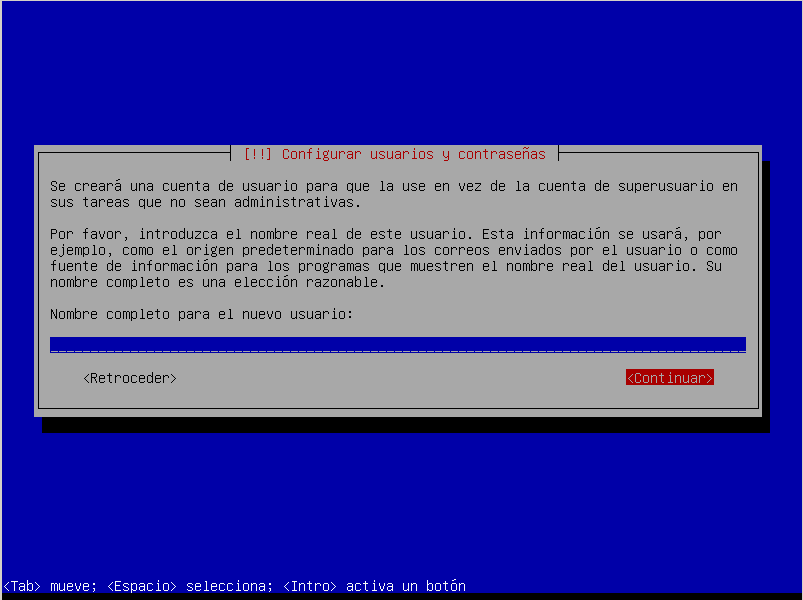
\includegraphics[ width=0.9\textwidth]{./imgs/4_7_install_new_user.png}
  \column{.5\linewidth}
                        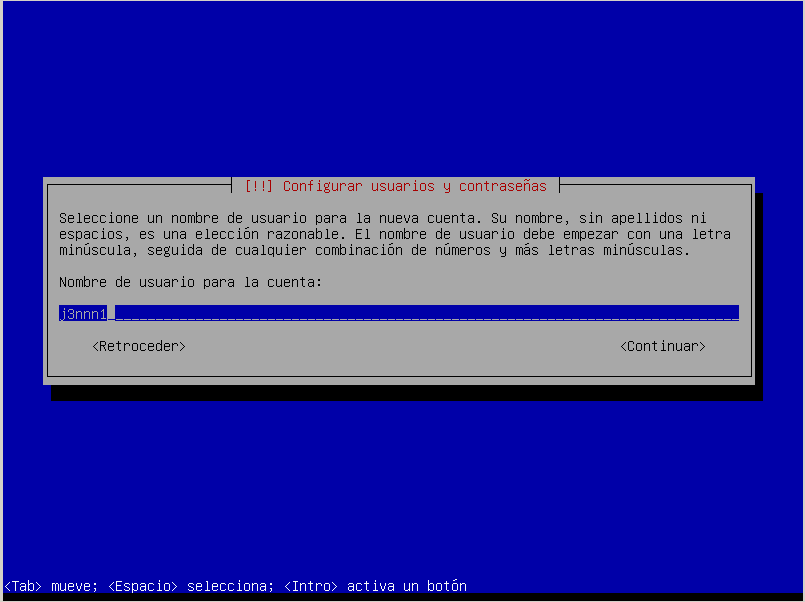
\includegraphics[ width=0.9\textwidth]{./imgs/4_8_install_confirm.png}
  \end{columns}
\end{frame} 

\subsection{Configuraci\'on general: Hora del sistema}
\begin{frame}
\frametitle{Usuario Personal y Hora del sistema} 
  \begin{columns}
  \column{.5\linewidth}
                        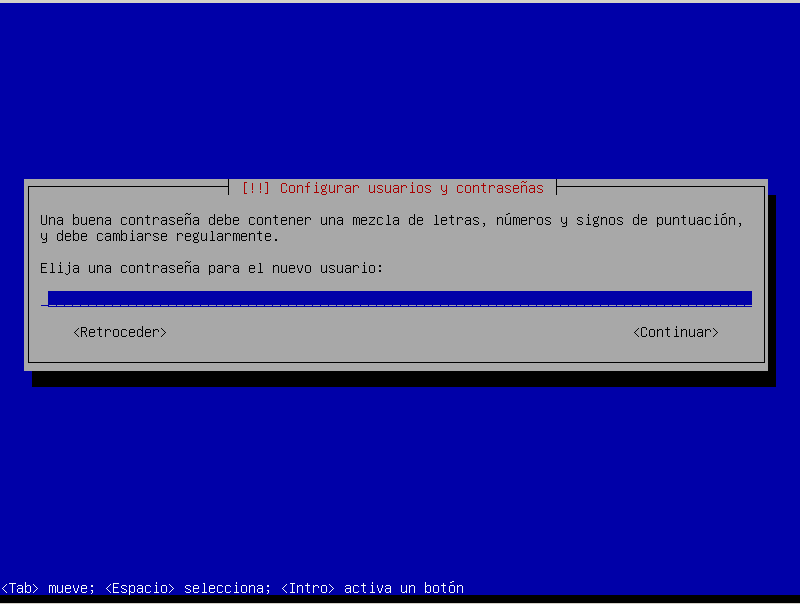
\includegraphics[ width=0.9\textwidth]{./imgs/4_9_install_config_pass_new_user.png}
  \column{.5\linewidth}
                        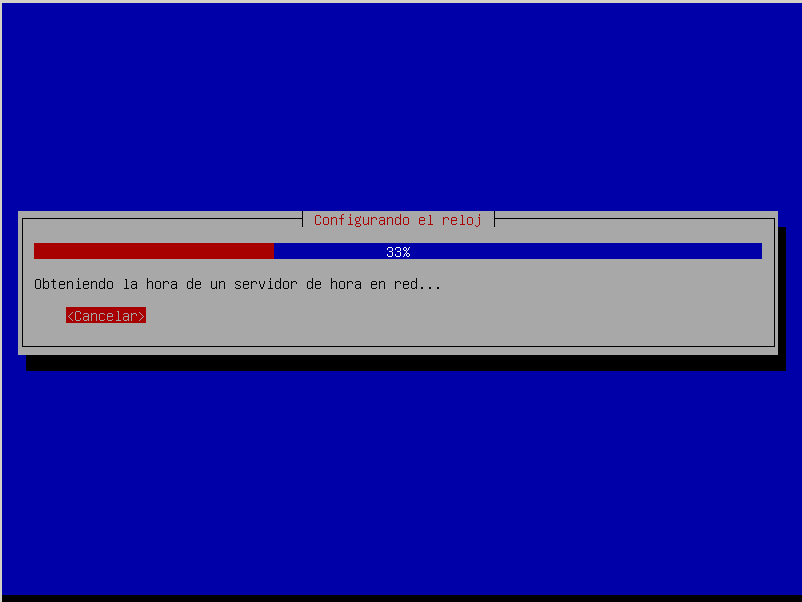
\includegraphics[ width=0.9\textwidth]{./imgs/4_10_install_obteniendo_hora.png}
  \end{columns}
\end{frame} 


\subsection{Configuraci\'on general: Particionamiento}
\begin{frame}
\frametitle{Particionamiento} 
                        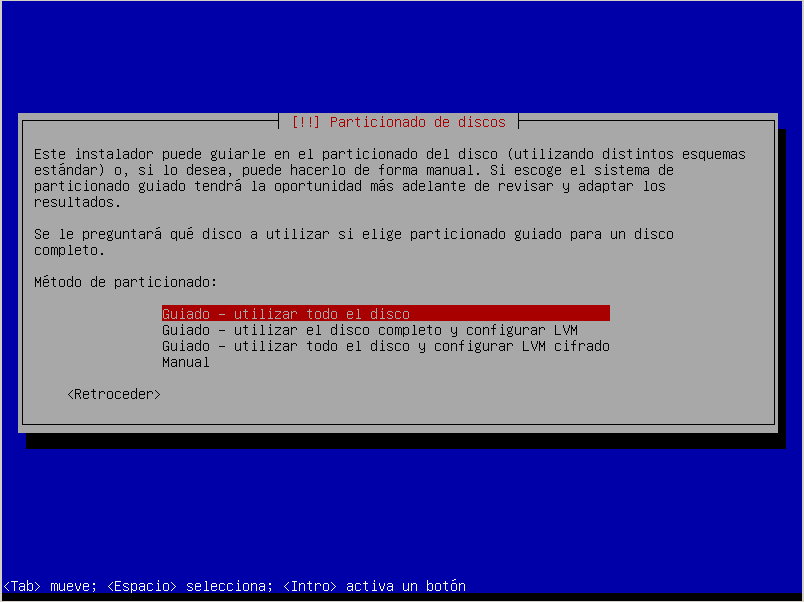
\includegraphics[ width=0.9\textwidth]{./imgs/4_11_install_comenzando_particionamiento.png}
\end{frame} 

\subsection{Configuraci\'on general: Particionamiento II}
\begin{frame}
\frametitle{Recuerda... sobre el particionamiento}
\begin{itemize}
\item Por lo general un disco s\'olo soporta 4 particiones, soporta m\'as particiones a trav\'es del particionamiento extendido.
\item El esquema de particionamiento puede ser sencillo de las siguiente forma:
\begin{itemize}
\item \alert{Separando Archivos Personales:} una partici\'on primaria para la ra\'iz o root  (/), una partici\'on para los archivos del usuario (/home) y una partici\'on de swap (\'area de intercambio)
\item \alert{Sencilla :} una partici\'on primaria para la ra\'iz o root  (/) y una partici\'on de swap (\'area de intercambio)
\item \alert{DualBoot :} una partici\'on primaria para el SO (windows), una partici\'on primaria para root (/), una partici\'on extendida que contenga /home y /swap
\end{itemize}
\item Las particiones que contienen al sistema linux pueden ser l\'ogicas, sin embargo si van a utilizar otro SO (windows) la partici\'on donde se encuentre este, tiene que ser primaria y debe chequeada para bootear.
\end{itemize}
\end{frame}

\begin{frame}
\frametitle{ Particionamiento}
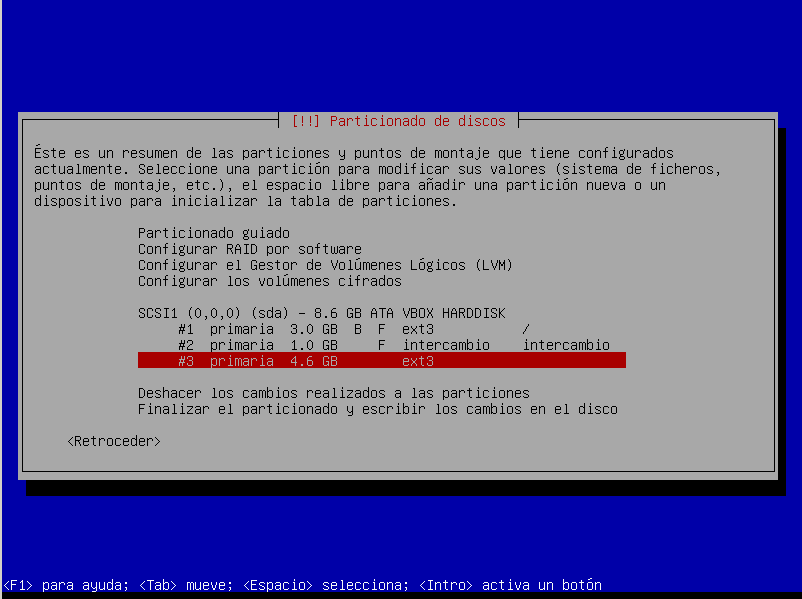
\includegraphics[ width=0.9\textwidth]{./imgs/installdebianparticion1.png}
\end{frame}

\begin{frame}
\frametitle{ Configurando Repositorios y gestor de Paquetes}
\begin{columns}
\column{.5\linewidth}
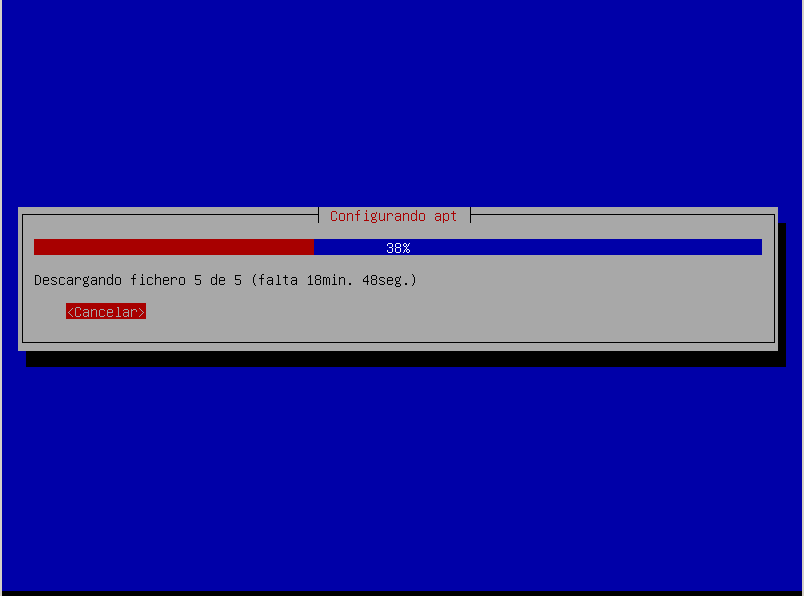
\includegraphics[ width=0.9\textwidth]{./imgs/instalandodebianrepositoriosred.png}
\column{.5\linewidth}
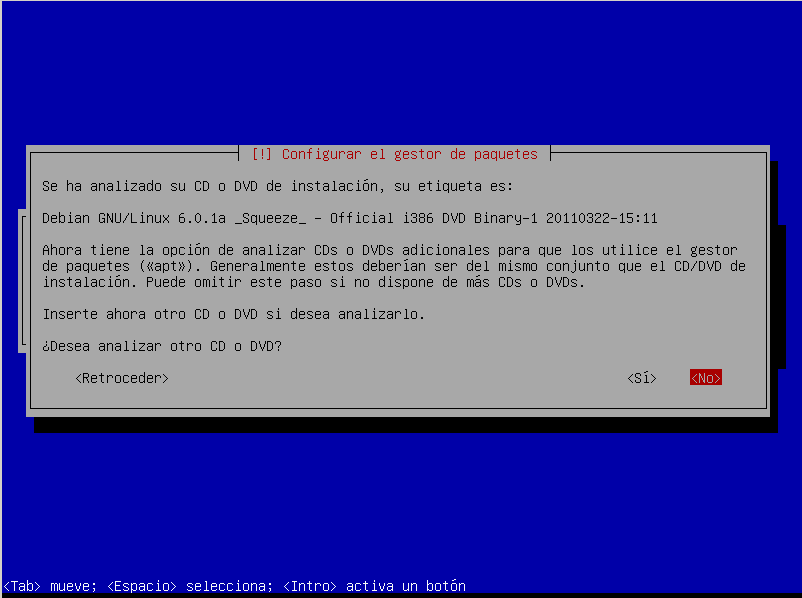
\includegraphics[ width=0.9\textwidth]{./imgs/installdebianconfiggestorpaquetes.png}
\end{columns}
\end{frame}


\begin{frame}
\frametitle{ Instalando sistema Base}
\begin{columns}
\column{.5\linewidth}
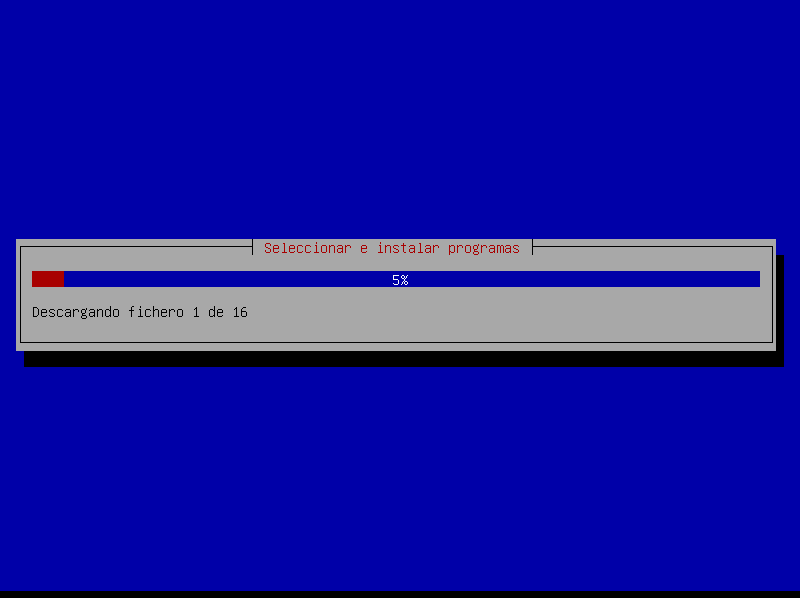
\includegraphics[ width=0.9\textwidth]{./imgs/instalaciondebianprogramas.png}
\column{.5\linewidth}
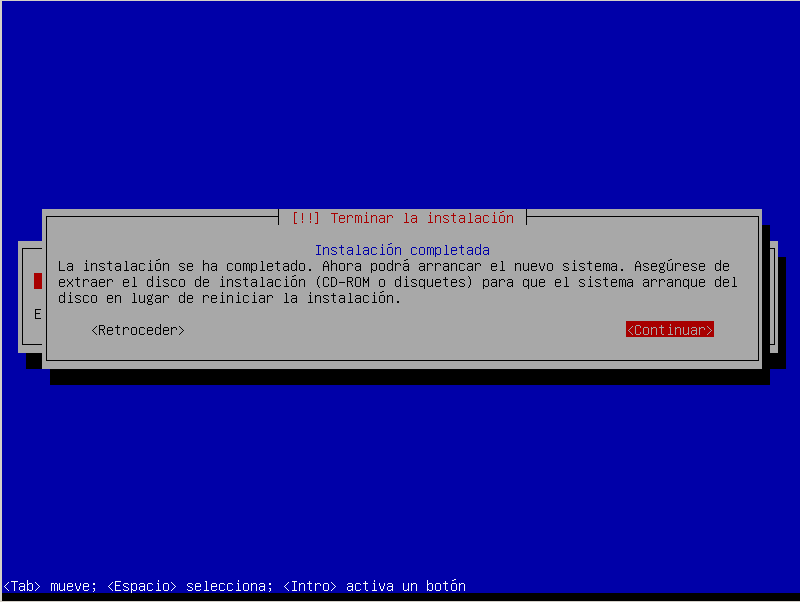
\includegraphics[ width=0.9\textwidth]{./imgs/instalacionterminada.png}
\end{columns}
\end{frame}

\begin{frame}
\frametitle{Finalizando Instalaci\'on} 
\begin{columns}
\column{.5\linewidth}
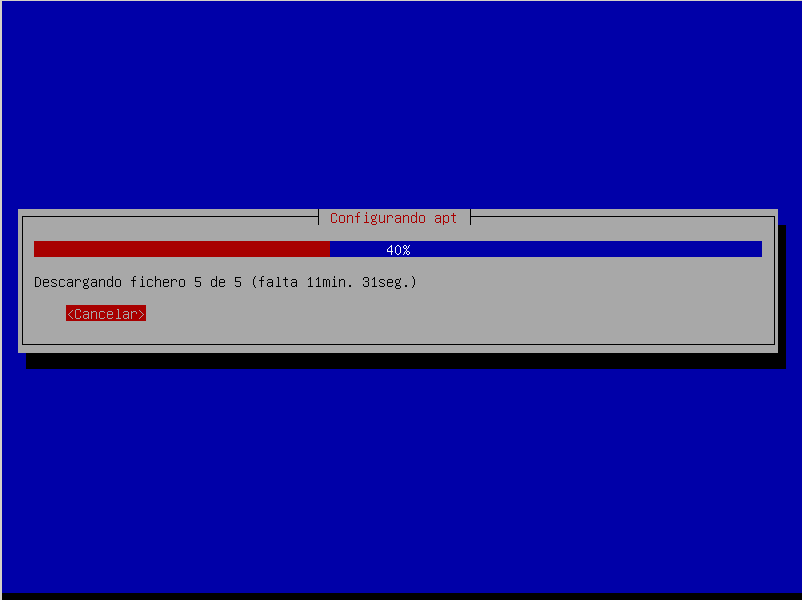
\includegraphics[ width=0.9\textwidth]{./imgs/instalandodebian.png}
\column{.5\linewidth}
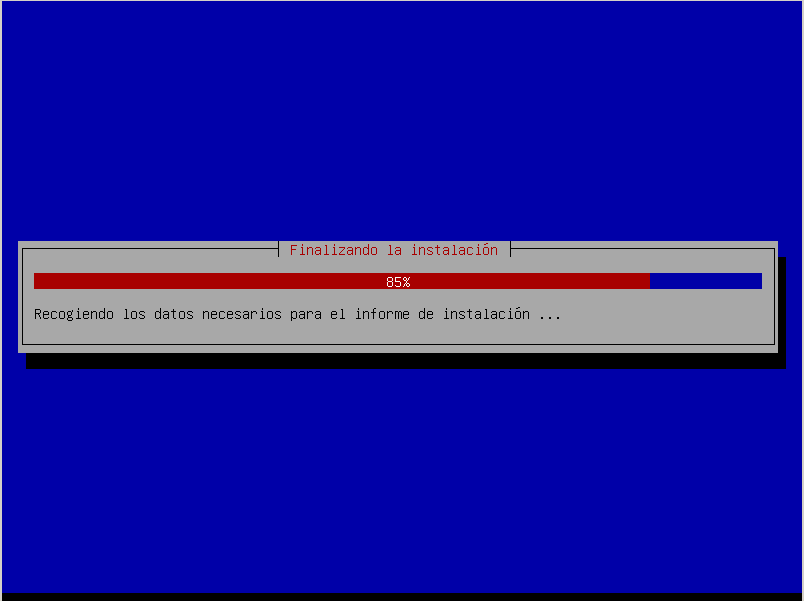
\includegraphics[ width=0.9\textwidth]{./imgs/finalizandoinstalaciondebian.png}
\end{columns}
\end{frame}

\subsection{Archivos de Configuraci\'on: Orígenes del Software}
\begin{frame}
\frametitle{Archivos de Configuraci\'on}
\begin{itemize}
	\item /etc/apt/sources.list (En Debian apt-setup, Ubuntu se encuentra en Or\'igenes de Software)
	\item /usr/share/doc/ (directorio donde encotraremos la documentaci\'on del sistema)
	\item /usr/local y /opt (software de terceros \'o instalado  manualmente)
	\item /etc/enviroment (variables de ambiente del sistema)
	\item /etc/hostname (nombre de la maquina)
\end{itemize}
\end{frame}

\subsection{Archivos de Configuraci\'on: Boot, Interfaz gráfica}
\begin{frame}
\frametitle{Archivos de Configuraci\'on}
\begin{itemize}
	\item /etc/fstab (archivo que muestra el listado de discos y particiones disponible, palabras claves: como y que configuraci\'on)
	\item /etc/X11/xorg.conf (archivo de configuraci\'on de la interfaz gr\'afica debian)
	\item /usr/share/X11/xorg.conf.d (UBUNTU)
	\item Xorg -configure / X -configure configuraci\'on por defecto del servidor gr\'afico
	\item /etc/grub.conf
\end{itemize}
\end{frame}

\subsection{Archivos de Configuraci\'on: Archivos de Configuración de Red}
\begin{frame}
\frametitle{Archivos de Configuraci\'on}
\begin{itemize}
	\item /etc/resolv.conf
	\item /etc/hosts
	\item /etc/networks/interface (interfaces de red)
	\item /boot/grub/grub.cfg (grub 2)
	\item /boot/grub/menu.lst (grub 1)
\end{itemize}
\end{frame}

\subsection{Archivos de Configuraci\'on: Usuarios}
\begin{frame}
\frametitle{Archivos de Configuraci\'on}
\begin{itemize}
	\item /etc/shadow (archivo de config del usuario)
	\item /etc/passwd (archivo de config del usuario)
	\item /etc/group (archivo de config de los grupos)
	\item /etc/deluser.conf 
	\item /etc/adduser.con 
	\item /etc/skel
\end{itemize}
\end{frame}

\section{Configuraci\'on}
\subsection{Configuraci\'on de Hardware}
\begin{frame}
\frametitle{La configuraci\'on}
\begin{itemize}
\item \alert{dpkg-reconfigure xserver-xorg} Por lo general cuando el sistema no detecta alguna tarjeta de video, se tienen la opcion del driver general VESA
\item \alert{/etc/network/interface}
\begin{itemize}
	\item Cuando el driver no se encuentra empaquetado por la distribución, o no es soportado.
	\item se requiere compilarse manualmente y añadirse al kernel.
	\item \alert{ndiswrapper}
	\item \alert{modprobe, rmmod, lsmod}
	\item \alert{drivers de video, ati, por defecto se utiliza vesa}
	\item \alert{alsa, alsa-mixer, alsa-utils}
	\item Muchas veces se requiere a\~nadir los usuarios a grupos para que puedan accder a los servicios.
	\item Ejemplo: para tener acceso al audio, red, impresora.. para cada dispositivo existe un grupo.
\end{itemize}
\end{itemize}
\end{frame}

\section{Agregar o Quitar Programas}
\subsection{Configuraci\'on de Software}
\begin{frame}
\frametitle{Herramientas  gr\'aficas}
\begin{itemize}
\item Aptitude
\item synaptic
\item KPackageKit
\item Muon Suite
\item PackageKit
\item Ubuntu Software Center
\end{itemize}
\end{frame} 


\subsection{Herramientas NO gr\'aficas}
\begin{frame}
\frametitle{Herramientas NO gr\'aficas}
	\begin{itemize}
	\item por defecto Debian trae instalado Aptitude.
	\item Ubuntu s\'olo apt-get
	\item Instalar nuevos programas.
		\begin{itemize}
			\item \alert{aptitude search  NombrePaquete}
			\item \alert{apt-get install NombrePaquete}
			\item \alert{aptitude install NombrePaquete}
			\item  dpkg -l
			\item  dpkg -i skype.deb o NombrePaquete.deb
			\item \alert {alien:} alien --to-deb /path/to/file.rpm
			\item A trav\'es de la fuente tarball tar.gz
		\end{itemize}
	\item Desintalar programas.
		\begin{itemize}
			\item \alert{Aptitude:}aptitude remove NombrePaquete
			\item \alert{apt-get:}apt-get remove NombrePaquete
			\item \alert{dpkg:}dpkg -r VMware-workstation 
			\item dpkg-reconfigure  xserver-xorg (configurar paquete, del servidor X)
			\item dpkg-reconfigure  locales
		\end{itemize}
	\end{itemize}
\end{frame} 

\subsection{Actualizaciones del Sistema}
\begin{frame}
\begin{itemize}
\frametitle{Actualizaciones del Sistema}
\item Actualizaciones y Parches de seguridad.
	\begin{itemize}
		\item \alert {aptitude update}
		\item aptitude safeupgrade o aptitude dist-upgrade (esto último es un alias)
                \item apt-get update
		\item apt-get dist-upgrade
        \end{itemize}
\item Administrando repositorios.
        \begin{itemize}
                \item /etc/sources.list
        \end{itemize}
\end{itemize}
\end{frame}

\section{Administraci\'on b\'asica del sistema: usuarios, archivos, tareas programadas. }
\subsection{usuarios}
\begin{frame}
\frametitle{A\~nadiendo usuarios}
\begin{itemize}
\item useradd (En Debian y Ubuntu, existe el script adduser deluser addgroup)
\item userdel (--remove-all-files) 
\item usermod
\item whoami - groups
\item who
\item id
\end{itemize}
\end{frame}

\section{Administraci\'on b\'asica del sistema: usuarios, archivos, tareas programadas. }
\subsection{usuarios}
\begin{frame}
\frametitle{A\~nadiendo usuarios a grupo}
\begin{itemize}
\item useradd usuario grupo 
\item usermod -g grupo usuario
\item usermod  -G listadodegrupos
\item passwd usuario (permite cambiar la clave del usuario)
\item passwd -d ventas (permite cambiar la clave al grupo de ventas)
\item passwd -g -r ventas (permite quitar la clave al grupo de ventas)
\item delgroup usuario grupo
\end{itemize}
\end{frame}

\subsection{Administraci\'on de usuarios}
\begin{frame}
\frametitle{Usuarios y grupos}
        \begin{itemize}
        \item gpasswd -a usuario grupo
        \item gpasswd -d usuario grupo
        \item groupadd grupo
        \item groupdel grupo
        \item groupmod admin -m newmember
        \item chgrp [-R] grupo archivo
        \item chown [-R] usuario archivo / chown [-R] usuario:grupo archivo
        \end{itemize}
\end{frame} 

\section{Administraci\'on b\'asica del sistema: usuarios, archivos, tareas programadas. }
\subsection{usuarios}
\begin{frame}
\frametitle{A\~nadiendo usuarios}
\begin{itemize}
\item su <usuario>
\item sudo (/etc/sudoers)
\item No dudes consultar info - man (En caso de duda..)
\end{itemize}
\end{frame}

\subsection{Administraci\'on de usuarios}
\begin{frame}
\frametitle{Usuarios y grupos}
\begin{itemize}
        \item Estructura del Archivo /etc/passwd.
                \begin{itemize}
                \item Login del usuario.
                \item x si existe password en el /etc/shadow.
                \item UID
                \item GID
                \item GECOS, (General Comprehensive Operating System \'o General Electric Comprehensive Operating Supervisor)
                \item directorio HOME
                \item Shell de inicio
                \end{itemize}
\end{itemize}
\end{frame}


\subsection{Administraci\'on de usuarios}
\begin{frame}
\frametitle{Administraci\'on de usuarios}
\begin{itemize}
\item Estructura del Archivo /etc/shadow
        \begin{itemize}
        \item Login del usuario
        \item password encriptado
        \item d\'ias transucrrido desde 1970 del \'ultimo cambio de password.
        \item M\'inimo de d\'ias antes que el password pueda ser cambiado.
        \item M\'aximo de d\'ias para cambiar el password.
        \item D\'ias de advertencias antes de que el password expire.
        \item D\'ias despues de expirado un password cuando la cuenta sea deshabilitada.
        \item D\'ias transcurridos desde 1-1-1970 en que ha estado deshabilitada.
        \item Reservado por sistema
        \end{itemize}
\end{itemize}
\end{frame}

\subsection{Permisolog\'ia en los archivos}
\begin{frame}
\frametitle{Permisolog\'ia en los archivos}
        \begin{itemize}
        \item S\'olo el propietario del archivo puede cambiar su permiso de acceso.
        \item chmod
        \item c\'alculo de forma octal para representar con bits los permisos
                \begin{itemize}
                        \item Debemos saber el valor de bits para cada acci\'on, lectura 4 escritura 2 ejecuci\'on 1
                        \item el primer valor es para el usuario due\~no del archivo, el segundo valor es para el grupo, y el tercer valor para otros.
                        \item \alert {Ejemplo: } chmod 777 archivo, chmod 644 archivo, chmod 755 archivo, chmod 751 archivo
                \end{itemize}
        \end{itemize}
\end{frame}

\begin{frame}
\begin{itemize}
\frametitle{Permisolog\'ia en los archivos}
\item Mediante comandos simb\'olico o  letras
\begin{itemize}
\item r (lectura), w (escritura), x (ejecuci\'on)
\item u (usuario), g (grupo) ,o (otros)
\item + (a\~nadir),  - (eliminar),  = (mantener)
\item \alert{Ejemplo:} chmod [ugo] [+-=] [rwx] Archivo.txt
\item chmod uog-xw+r permiso.txt, chmod +x archivo.txt
\end{itemize}
\end{itemize}
\end{frame}

\begin{frame}
\frametitle{Permisos de Directorios}
\begin{itemize}
\item r puede leer la lista de directorios (no implica que se pueda acceder a los archivos)
\item w puede escribir en el directorio (crear, renombrar y borrar archivos)
\item x puede buscar en el directorio (entrar y acceder a los archivos)
        \begin{itemize}
        \item para leer, escribir, y crear un archivo, el directorio debe tener el permiso de ejecuci\'on x
        \end{itemize}
\end{itemize}
\end{frame}


\subsection{Permisos Adicionales.}
\begin{frame}
\frametitle{Permisos Adicionales.}
\begin{itemize}
	\item \alert{set user ID,  SUID:} cambio de clave de un usuario, quien ejecute /bin/passwd se enmascara en el usuario due\~no de este binario, para poder modificar el archivo /etc/passwd, ya que cómo usuario normal no podría hacerlo directamente.
	\item -rwsr-xr-x 1 root root 24704 jun 26 02:42 /usr/bin/passwd - SUID valor octal 4
	\item \alert{set group ID,  SGID:}  En este caso al ejcutar el binario, se enmascarar\'a con el id del grupo. el valor octal GUID es 2
	\item find / -perm -4000 -o -perm -2000 -print 
	\item \alert{sticky bit:} hace que un archivo o directorio no sea borrable, renombrable, o permitan mover los archivos de su estado, aún cuando el usuario tenga permisos sobre ese directorio o archivo, queda exceptuado el dueño del archivo y root.
	\item find / -perm 1000 -print
\end{itemize}
\end{frame}

\subsection{Ambiente y variables de entorno}
\begin{frame}
\frametitle{Ambiente y variables de entorno}
        \begin{itemize}
                \item PATH contiene los directorios en los cuales se encuentran los binarios.
                \item HOME ruta de la carpeta de archivos personales.
                \item DISPLAY contiene el identificador del display que los programas del servidor X deben usar por defecto.
                \item RANDOM, arroja un numero pseudo aleatorio, cada vez que se utiliza.
                \item LANG, contiene el locale (juego de caracteres que caracterizan un idioma o localidad) por defecto del sistema, tiene relacion LC\_ALL  ignorar el contenido de la variable LANG.
        \end{itemize}
\end{frame}

\begin{frame}
\frametitle{Ambiente y variables de entorno}
	\begin{itemize}
		\item LC\_COLLATE : Controla la forma de clasificar: que letras van antes y despu\'es de otras en orden alfab\'etico.
		\item LC\_CTYPE: Controla la correspondencia entre letras may\'usculas y min\'usculas adem\'as de definir los componentes de las diferentes clases de caracteres, como los caracteres alfanum\'ericos. 
		\item SHELL imprime el tipo de shell que se est\'a usando. HISTFILE, nombre del archivo donde se almacenaran los comandos ejecutados.
		\item USER, USERNAME, imprime el nombre del usuario. HOSTNAME, nombre del sistema.
		\item OSTYPE, tipo de sistema operativo ejecutandose. HTTP\_PROXY, indica la ip, o nombre del servidor proxy.
		\item comandos para manejo del entornos de variables:
		\begin{itemize}
		\item set ,env,  export, unset
		\item Ejemplo:  export VARIABLE=VALOR, set VARIABLE=VALOR, unset VARIABLE.
		\end{itemize}
	\end{itemize}
\end{frame}

\subsection{Ambiente y variables de entorno}
\begin{frame}
\frametitle{Ambiente y variables de entorno}
        \begin{itemize}
                \item Variables atadas una terminal
		\begin{itemize}
			\item Estos archivos contienen configuraci\'on asociada a la shell que utilizamos, y aplica para todos los usuarios.
			\item /etc/profile
			\item /etc/bash.bashrc
			\item para que las variables solo afecten a un usuario en espec\'ifico deben ser modificados los archivos de configuraci\'on que se encuentran en el directorio personal del usuario. e.g. ~/.bashrc
		\end{itemize}
		\item Afectan a Todo el sistema, no a un usuario en particular y no están atadas a una terminal
			\item /etc/enviroment
        \end{itemize}
\end{frame}

\subsection{Metacaracteres}
\begin{frame}
\frametitle{ Metacaracteres }
	\begin{center}
	\begin{tabular*}{\textwidth}{ @{\extracolsep{\fill}}  | l | c |  }
		\hline
		car\'acter & descripci\'on  \\	
		\hline
		* & {\tiny  uno o m\'as caracteres, es decir a cualquier caracter en nombre de archivo. } \\	
		\hline
		\& & {\tiny Ejecuta un proceso en segundo plano.} \\	
		\hline
		\textgreater \'o \textless \'o \textless \textless \'o \textgreater \textgreater & {\tiny Redirecciona la salida a un archivo.} \\	
		\hline
		\$ & {\tiny Extrae el contenido de una variable.} \\	
		\hline
		\&\&  & {\tiny Condicional AND } \\	
		\hline
		| |  & {\tiny  Condicional OR} \\	
		\hline
	\end{tabular*}
	\end{center}
\end{frame}

\subsection{Sentencias y Comandos}
\begin{frame}
\frametitle{Sentencias y Comandos}
\begin{itemize}
\item \alert{Ejecutar comandos}: llamada directa al ejecutable, a trav\'es de una variable de entorno, a trav\'es de un alias.
\item \alert{Separar comandos}: pueden ser separados por (;) , por un backslash ( $\backslash$ ), y colocando cada comando en una l\'inea.
\item \alert{Entrada y Salida Estandar}:
	\begin{itemize}
	\item Entrada Estandar (Teclado), 1 Salida Estandar (Muestra por pantalla ) , 2 Salida de Errores (Salida destinada a los errores o depuraci\'on)
	\item Ejemplo: ls -l | cat \textgreater \textgreater archivo.txt \'o script 2 \textgreater \textgreater archivo.txt \'o   script-programa \textgreater fichero 2\textgreater\&1
	\end{itemize}
\end{itemize}
\end{frame}


\subsection{Archivos de bit\'acoras}
\begin{frame}
\frametitle{Archivos de Bit\'acora}
\begin{itemize}
\item /var/log/Xorg.0.log
\item /var/log/zypper.log
\item /var/log/messages
\item /var/log/lastlog
\item /var/log/firewall
\item /var/log/mail
\item /var/adm/syslog.log \'o /var/log/syslog.log
\end{itemize}
\end{frame}

\subsection{Utilizado en clase}
\begin{frame}
\frametitle{Buscar informaci\'on en Bit\'acoras}
\begin{itemize}
\item \alert{tail}: tail -f archivo, tail -n30, lista las \'ultimas l\'ineas de un archivo.
\item \alert{head}: head -n40, lista las primeras l\'ineas de un archivo.
\item \alert{cat}: permite combinar o concatenar varios archivos, en caso de un solo archivo muestra todo su contenido.
\item \alert{less}: paginador de textos, q para salir, y con las flechas de navegaci\'on del teclado puedes recorrer el texto.
\item \alert{more}: paginador de textos, q para salir, y con tabulador se desplaza.
\\
\item ls -l | (less/more), tail -n100 | grep "Patr\'onABuscar" | (less/more).
\end{itemize}
\end{frame}

\subsection{Herramientas}
\begin{frame}
\frametitle{Herramientas}
B\'usqueda de informaci\'on:  find, grep, locate, sort, cat, egrep, tail, head, wc, xarg.
Monitoreo de Redes: netstat, traceroute, ping.
Monitoreo local: free, df, last, lastlog, pstree, ps, uptime, top, dmesg.
Chequeo y Administraci\'on: watch, md5sum, zypper, rpm, diff.
\end{frame}

\subsection{Los Procesos.}
\begin{frame}
\frametitle{Los Procesos.}
\begin{defi}
Es un programa/comando/shellscript que se est\'a ejecutando en memoria, cuando el proceso es finalizado se elimina de memoria. cada proceso tiene un Id que lo identifica como \'unico.
\end{defi}
\end{frame}

\subsection{Tipos de Procesos.}
\begin{frame}
\frametitle{Tipos de Procesos.}
\begin{itemize}
\item Background (Segundo Plano), Procesos iniciados por el sistema, como demonios a trav\'es del  script de arranque por lo general.
\item Foreground (Primer Plano), son procesos iniciados desde una c\'onsola por un usuario, tambi\'en se les dice procesos con contrl de terminal.
\end{itemize}
\end{frame}

\subsection{Los Procesos.}
\begin{frame}
\frametitle{Los Procesos.}
\begin{itemize}
\item Listando procesos: ps aux, a selecciona todos los procesos no asociados a una terminal, u despliega formato orientado al usuario, x procesos asociados a una terminal.
\end{itemize}
\end{frame}

\subsection{Comandos para el Control de Procesos}
\begin{frame}
\frametitle{Comandos para el Control de Procesos.}
\begin{itemize}
\item ps permite desplegar los procesos actuales.
\item pstre muestra el \'arbol de procesos.
\end{itemize}
\end{frame}

\subsection{ Monitoreo para el control de Proceso.}
\begin{frame}
\frametitle{Monitoreo para el control de Proceso.}
\begin{itemize}
\item top: es un comando c\'iclico que ordena los primeros 20 procesos, htop (interfaz humana).
\item free: permite ver el uso de la memoria f\'isica y compartida.
\item uptime: tiempo transcurrido desde que se inici\'o la computadora.
\end{itemize}
\end{frame}


\subsection{Comandos para el Control de Procesos}
\begin{frame}
\frametitle{Comandos para el Control de Procesos.}
\begin{itemize}
\item jobs: lista los procesos ejecutandose en background
\item kill: se usa para enviar se\~nales a procesos en ejecuci\'on. Ejemplo: kill \textless se\~nal \textgreater PID, kill -l (lista las se\~nales disponibles), kill -SIGTERM 12345, kill -15 12345.
\item bg, fg: Se usa para enviar procesos detenidos al modo background, y fg se usa prar enviar los procesos ejecut\'andose en background al modo foreground.
\item nice: te permite asignar prioridad a un proceso, antes de ejecutarse. Ejemplo: nice 19 procesoaEjecutar.
\item renice:  te permite modificar el valor de la prioridad a los procesos luego de iniciarlo, o estando en ejecuci\'on. Ejemplo:  renice 18 PID.
\end{itemize}
\end{frame}

\subsection{Utilizando kill}
\begin{frame}
\frametitle{Utilizando kill}
\begin{itemize}
\item kill -9 NROPROCESO
\item kill -SIGTERM NROPROCESO
\item kill -1 NROPROCESO
\item kill -HUP NROPROCESO (Procesos Zombie)
\item kill -15 NROPROCESO (Terminaci\'on de un proceso)
\end{itemize}
\end{frame}

\subsection{Procesos Agradables..}
\begin{frame}
\frametitle{Procesos Agradables..}
\begin{itemize}
\item El valor de nice puede variar de -19 a 19, siendo el m\'as negativo con mayor prioridad (es el m\'as desagradable) a medida que el valor es positivo tiene menor prioridad de procesamiento.
\item Solo puedes modificar la prioridad de procesos si le pertenecen al usuario, a menos que sea root.
\item nice 10 BINARIOAEJECUTAR
\item renice 15 PID (N\'umero de Proceso)
\end{itemize}
\end{frame}


\subsection{Agendar Ejecuci\'on de Procesos.}
\begin{frame}
\frametitle{Agendar Ejecuci\'on de Procesos.}
\begin{itemize}
\item Son procesos iniciados por el demonio Cron, pueden ser recurrentes de forma diaria, semanal o mensual, o de una sola ejecuci\'on.
\item Archivos de configuraci'on:
        \begin{itemize}
        \item General /etc/crontab
        \item Por Usuario: /var/spool/cron/tabs/usuario
        \end{itemize}
\end{itemize}
\end{frame}

\subsection{Agendar Ejecuci\'on de Procesos.}
\begin{frame}
\frametitle{Agendar Ejecuci\'on de Procesos.}
\begin{itemize}
\item Estructura del Archivo crontab (crontab -e)
        \begin{itemize}
        \item Minutos (0-59)
        \item Horas (0-23)
        \item D\'ias (1- 31)
        \item Meses (1-12)
        \item Dia-de-Semana (1-7)
        \item usuario de Ejecuci\'on
        \item comando a ejecutar
        \end{itemize}
\item El Entorno de variables en cron es diferente al establecido por /etc/profile, /etc/bash\_bashrc.
\item crontab -l : lista las entradas del crontab
\item crontab -r :elimina el crontab que ya existe.
\end{itemize}
\end{frame}

\subsection{Directorios para Ejecuci\'on periodica.}
\begin{frame}
\frametitle{Directorios para Ejecuci\'on periodica.}
\begin{itemize}
\item /etc/cron.hourly
\item /etc/cron.daily
\item /etc/cron.weekly
\item /etc/cron.montly
\item Ejemplo: 22 4 * * 0 root comand
\end{itemize}
\end{frame}

\subsection{Introducci\'on a los niveles de Ejecuci\'on}
\begin{frame}
\frametitle{Introducci\'on a los niveles de Ejecuci\'on (Proceso de Arranque en Linux)}
\begin{itemize}
\item Al iniciar un SO linux existe una secuencia de arranque, comenzando por la BIOS al verificar los dispositivos, luego la BIOS si existe alg\'un programa instalado en el MBR lo ejecuta, En este caso encontraremos al GRUB (o gestor de arranque preferido), el cual al inicializar nos muestras los diferentes SO disponibles, al seleccionar alguno disponible se monta en /boot, inicializa los dispositivos de memoria, carga controladores, monta el sistema de archivo / en modo lectura, y ejecuta el proceso init (Proceso padre), el proceso init lee el archivo de configuraci\'on /etc/inittab e inicia los script que corresponde al Nivel De Ejecuci\'on.
\end{itemize}
\end{frame}

\begin{frame}
\begin{itemize}
\frametitle{Introducci\'on a los niveles de Ejecuci\'on (Proceso de Arranque en Linux)}
\item \alert{Niveles de Ejecuci\'on} Es el modo de operaci\'on que implementan los sistemas Operativos basados en el sistema de arranque tipo Unix System V, Se podr\'ia definir como un estado en el que una serie de script se deben ejecutar.
\item Para todas las distribuciones los niveles de ejecuci\'on que no var\'ian son: runlevel 0 (Apagar) , runlevel 6 (reiniciar), 1 (monousuario).
\item Opensuse utiliza el nivel de ejecuci\'on 5 por defecto para mostrar su entorno gráfico.
\item Debian/Ubuntu utiliza el nivel de ejecuci\'on 2 por defecto para mostrar su entorno gráfico.
\end{itemize}
\end{frame}

\subsection{En Resumen}
\begin{frame}
\frametitle{En Resumen el Arranque...}
\begin{itemize}
	\item Arranque del Hardware
	\item Cargador del SO
	\item Puesta en marcha del Nucleo
	\item Init e inittab
	\item Scripts de inicio
\end{itemize}
\end{frame}

\subsection{Niveles de Ejecuci\'on}
\begin{frame}
\frametitle{Niveles de Ejecuci\'on}
\begin{itemize}
\item \alert{1}: Modo monousuario, permite hacer reparaciones en el sistema, no ejecuta demonios, ni configura la interfaz de red.
\item \alert{2}: Local multiuser without remote network, multiusuario sin configurar la interfaz de red. 
\item \alert{3}: Full multiuser with network, Multiusuario con acceso a red, sin interfaz gr\'afica.
\item \alert{4}: Not usado por la mayoría de las distribuciones
\item \alert{5}: Multiusuario con acceso a red, y con interfaz gr\'afica.
\item \alert{6}: Ejecuto los scripts de parada e inicio, para reiniciar el sistema.
\item \alert{0}: Ejecuta los scripts para el cierre del sistema.
\end{itemize}
\end{frame}

\subsection{Introducci\'on a los niveles de Ejecuci\'on}
\begin{frame}
\frametitle{Introducci\'on a los niveles de Ejecuci\'on}
\begin{itemize}
\item Los scripts de inicio en debian/ubuntu se encuentran en /etc/rc.d{0-6}
\item En el directorio anterior se encuentran enlaces simb\'olicos
\item Los scripts en estos directorios tienen una nomeclatura muy particular: EOrdenNombre, donde E puede ser una letra S (start, iniciar proceso) o  K (terminar proceso), Orden es el n\'umero de secuencia(orden de ejecuci\'on), y Nombre es el nombre del script de ejecuci\'on en el directorio /etc/init.d/rc{0-6}.d
\item comandos utilizados para el control de los niveles de ejecuci\'on: runlevel, init, telinit, shutdown, halt, reboot, chkconfig.
\end{itemize}
\end{frame}

\begin{frame}
\frametitle{Scripts de arranque}
\begin{itemize}
	\item Para cada servicio existe un script para su gesti\'on ubicado generalmente en /etc/init.d
	\item Usualmente llevan como parametro de entrada start|stop|restart
	\item Estos scripts son utilizados por los niveles de ejecuci\'on(/etc/rc{0-6S}.d).
\end{itemize}
\end{frame}

\section{Definiendo Archivo Inittab}
\begin{frame}
\frametitle{Definiendo Archivo Inittab}
\begin{itemize}
	\item id: identificador \'unico de una entrada en el archivo inittab
	\item niveles\_ejecuci\'on: especifica lista de niveles de ejecuci\'on para los cuales se llevar\'an  a cabo acciones espec\'ificas.
	\item acci\'on: acciones a realizar en un nivel de ejecuci\'on dado. Entre estas estan:
		\begin{itemize}
			\begin{columns}
			\column{.5\linewidth}
				\item respawn: 
				\item wait:
				\item once: 
				\item boot
				\item bootwait:
				\item off
				\item ondemand
			\column{.5\linewidth}
				\item initdefault:
				\item sysinit:
				\item powerwait:
				\item powerfail:
				\item ctrlaltdel
				\item kbrequest:
				\item proceso
			\end{columns}
		\end{itemize}
\end{itemize}
\end{frame}

\begin{frame}
\frametitle{A\~nadir un Servicio al Inicio}
\begin{itemize}
	\item \alert{update-rc.d dhcp3-server defaults} : A\~nade un servicio con parametros por defecto.
	\item update-rc.d ssh defaults
	\item update-rc.d ssh start 20 2 3 4 5 . stop 20 0 16 .
	\item update-rc.d ssh start 20 2 3 4 5 . stop 20 0 16 .
	\item \alert{update-rc.d -f dhcp3-server remove}: Elimina un servicio al iniciar el sistema, En resumen elimina los enlaces en el directorio rc.(n\'umero).d.
\end{itemize}
\end{frame}

\begin{frame}
\frametitle{Resumen...}
\begin{itemize}
 \item Cuando existe algun fichero con el nombre /etc/rc[nivel\_ejecucion]/SKNNombre update-rc.d no hace nada.
\item Para verificar que realizar\'ia el comando sin realizar los cambios, utilice la opci\'on -n. 
\item update-rc.d -n bluetooh defaults
\item update-rc.d -n -f bluetooh remove
\item Este programa debe ser ejecutado como administrador de sistemas o sudo.
\end{itemize}
\end{frame}

\subsection{Modificar Aplicaciones al inicio mediante Entorno Gr\'afico}
\begin{frame}
\frametitle{Modificar Aplicaciones al inicio mediante Entorno Gr\'afico}
	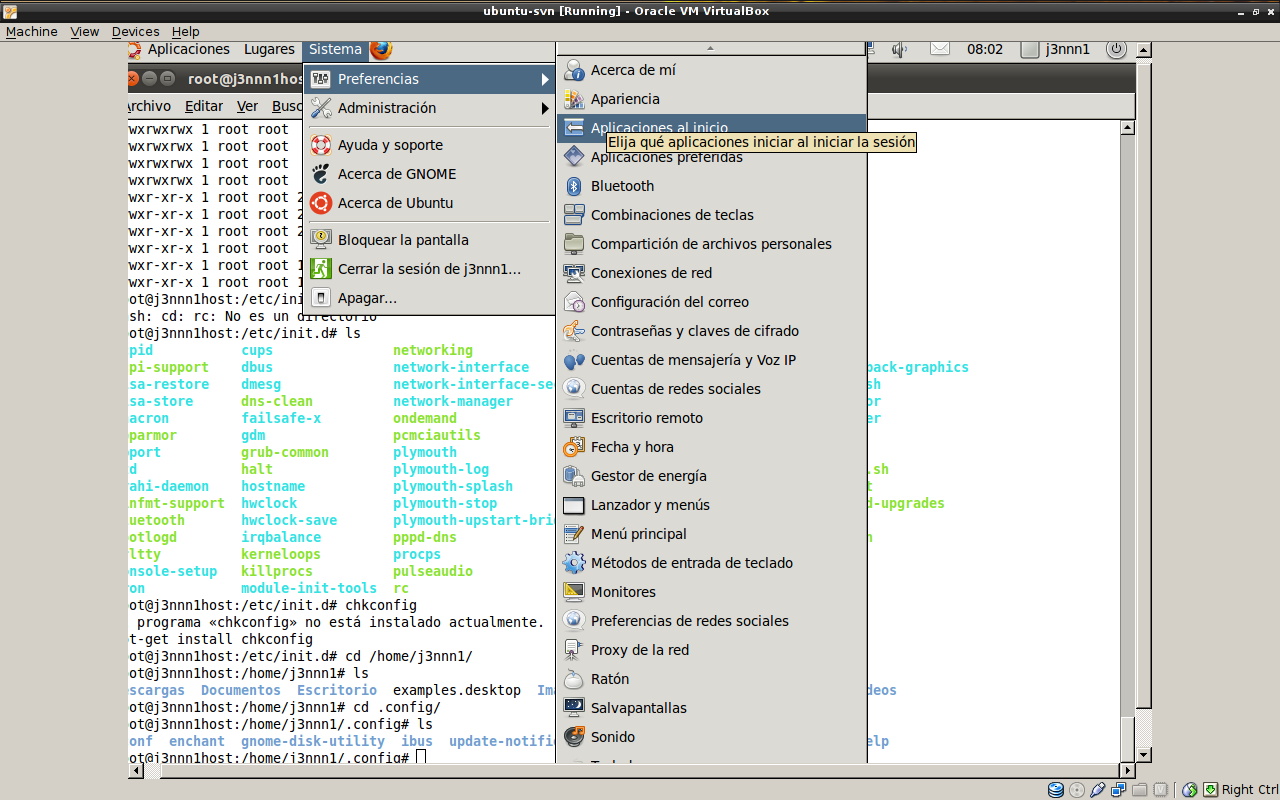
\includegraphics[height=0.5\textheight]{./imgs/inicio2.png} \hspace*{5.0cm}
\end{frame}

\begin{frame}
\frametitle{Modificar Aplicaciones al inicio mediante Entorno Gr\'afico}
	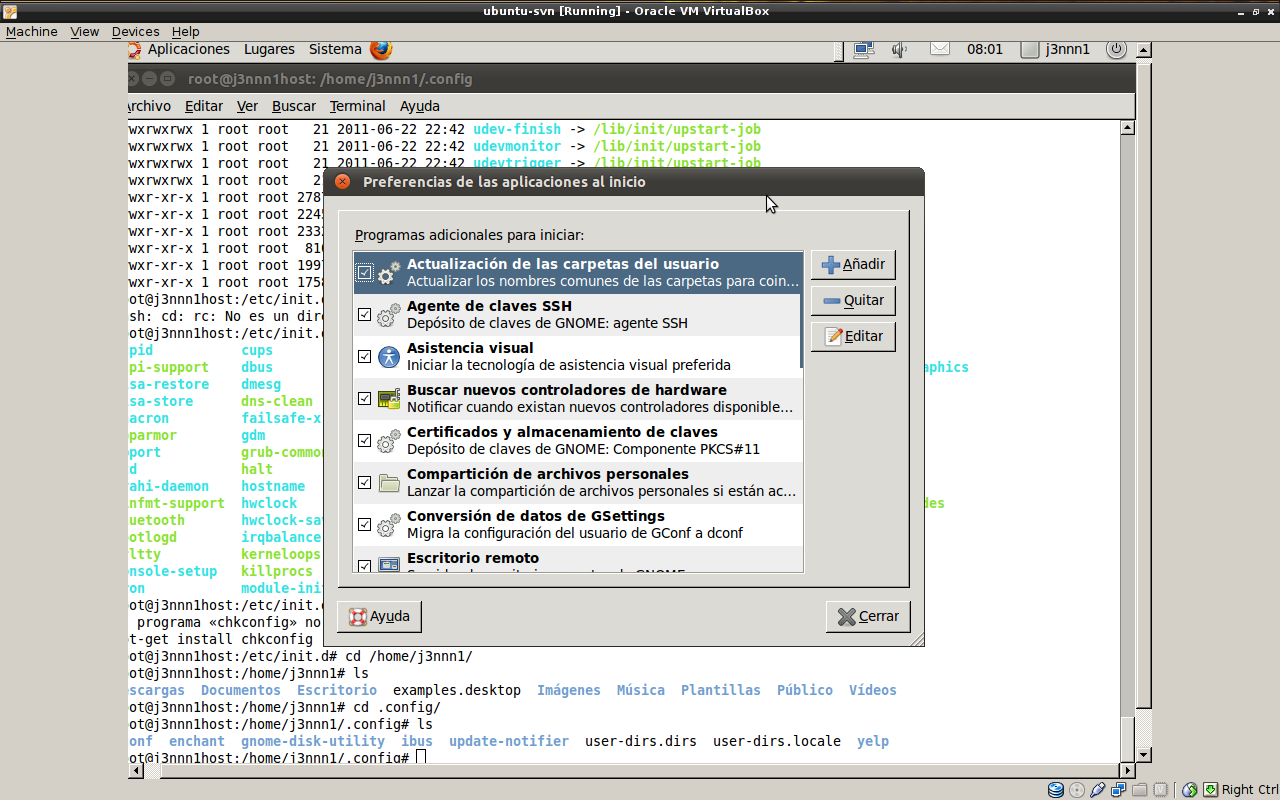
\includegraphics[height=0.5\textheight]{./imgs/inicio.png} \hspace*{1.0cm}
\end{frame}

\begin{frame}
\frametitle{Recetas vistas en clase}
\begin{itemize}
\item \alert{startx -- :2} Inicialia otro display para iniciar sesión de un usuario.
\item \alert{xinit /usr/bin/xterm -- :2} Inicialia otro display solo con el programa espec\'ifico
\item \alert{/etc/gdm/custom.conf} Login Autom\'atico en GDM, AutomaticLoginEnable=true, AutomaticLogin=miguel en la secci\'on de daemon, administracion->pantalla de acceso->iniciar sesion autom\'atica con el usuario curso, gdmsetup es la aplicacion backend que realiza estos cambios.
\item \alert{menu.lst /etc/grub.d/} Modificar el orden en el que aparecen los sistemas operativos, en este directorio se almacenan los archivos que crean una nueva entrada de booteo, lo que debe es modificarse el n\'umero que antecede el nombre del archivo, ejemplo 10\_os-probe se colocar\'a primero que 20\_linux y as\'i sucesivamente. Luego de realizar las modificaciones debe actualizarse mediante el comando: \alert{update-grub}
\end{itemize}
\end{frame}

\begin{frame}
\frametitle{Recetas vistas en clase}
\begin{itemize}
\item \alert{scp usuario@192.168.0.139:~/archivo.tar.gz .} Permite copiar un archivo de un host remoto a un host local a trav\'es del protocolo SSH
\item scp usuario@host:directorio/ArchivoOrigen ArchivoDestino
\item scp ArchivoOrigen usuario@host:directorio/ArchivoDestino
\item si se utiliza un sistema de archivos ntfs en alguna partici\'on y desean escribir en ella, tener en cuenta instalar ntfs-3g, 
\end{itemize}
\end{frame}

\begin{frame}
\frametitle{Referencias}
\begin{itemize}
\item http://www.linux-laptop.net/ 
\item http://linuxwireless.org/en/users
\item http://kmuto.jp/debian/hcl/index.cgi
\item http://www.x.org/releases/current/doc/man/man5/xorg.conf.5.xhtml
\item http://manpages.ubuntu.com/manpages/natty/es/man7/boot.7.html
\item http://manpages.ubuntu.com/manpages/hardy/es/man8/update-rc.d.8.html
\item man
\item info
\end{itemize}
\end{frame}
\end{document}
%%---End-Clase 1---------------------------------------
